
\begin{figure*}[t]
    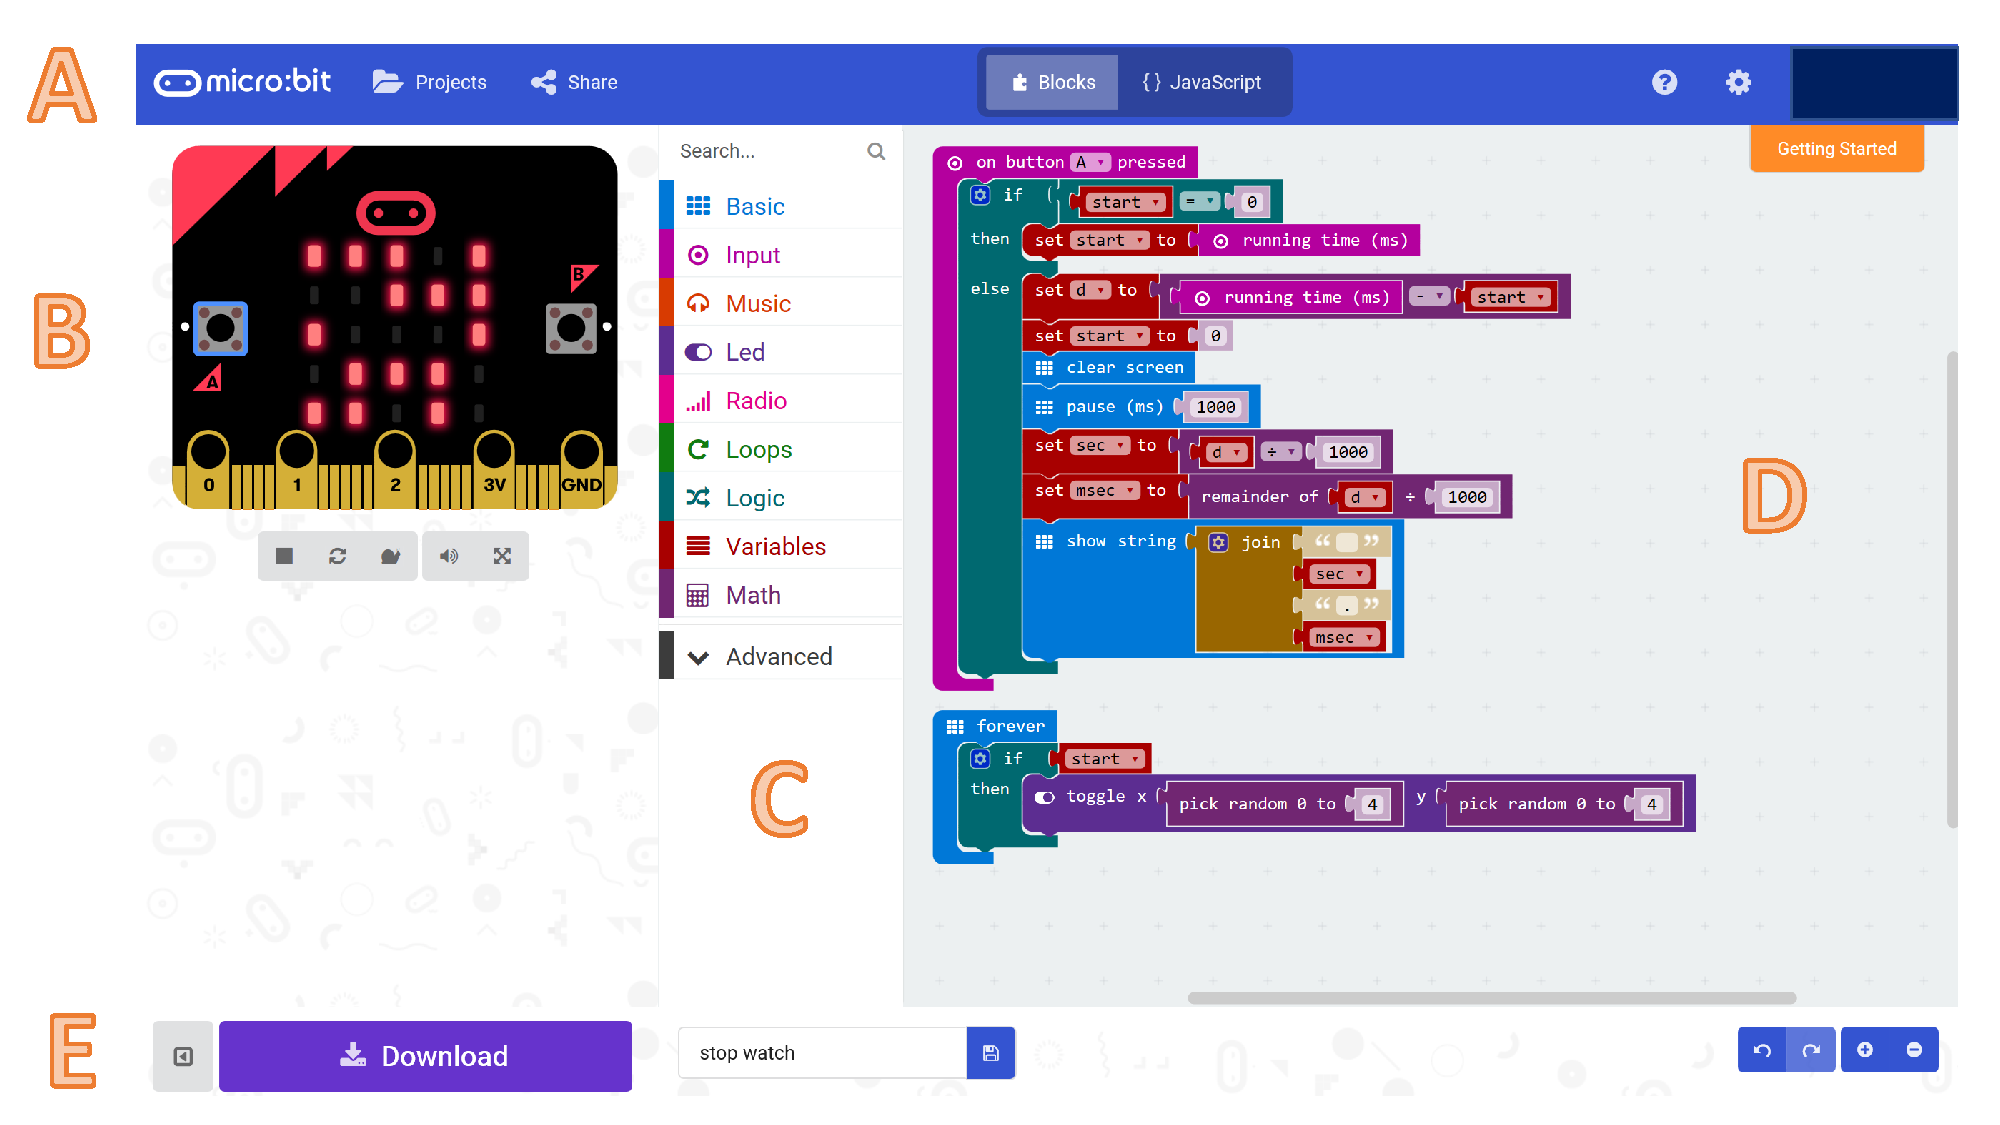
\includegraphics[width=5in]{screenSnapFig.pdf}
\caption{\label{fig:screenSnap}Screen snapshot of the \MC web app, showing the Blockly
view of the JavaScript from Figure~\ref{fig:example}.}
\end{figure*}


\section{\MCN: Design and Implementation}
\label{sec:makecode}

Figure~\ref{fig:screenSnap} shows a screen snapshot of the \MC web app for the micro:bit: 
(A) the menu bar allows switching between views of blocks and JavaScript;
(B) the simulator provides feedback on user code executed in the browser;
(C) the toolbar provides access to device-specific APIs and programming elements;
(D) the programming canvas (showing here the blocks corresponding to the JavaScript from Figure~\ref{fig:example});
(E) the download button invokes the compiler to produce a binary executable.

The \MC web app encapsulates all the components needed to deliver a programming experience 
for microcontrollers, free of the need for a C++ compiler for the compilation of user code.
The web app is written in TypeScript and incorporates the TypeScript compiler and 
language service as well. 
The app is built from a \MC ``target'' (\emph{\dbhref{https://github.com/microsoft/pxt-microbit}{pxt-microbit}})
which extends the \MC framework (\emph{\dbhref{https://github.com/microsoft/pxt}{pxt}}).
The remaining subsections describe the parts of Figure~\ref{fig:makecode}, 
which shows the high-level components of the web app.

\subsection{Device runtime and Shim Generation}

A \MC target is defined, in part, by its device runtime, which can be a combination of C++ 
and Static TypeScript (STS) code, as shown in the lower-left of Figure~\ref{fig:makecode}.
All C++ files for the target microcontroller are precompiled 
and stored in the cloud in a single blob and also is cached in the HTML5 application cache (with 
other assets) so that the web app can function when the browser is offline. Additional runtime
components may be authored in STS, which allows the device runtime to be updated without the
use of C++, and permits components of the device runtime to be shared by both the device
and simulator runtimes. The ability to author the device runtime in both STS and C++ is
a unique aspect of \MCN's design.

Whether runtime components are authored in C++ or STS, all runtime APIs are exposed as fully-typed
TypeScript definitions. A fully-typed runtime improves the end-user experience 
by making it easier to discover APIs; it also enables the type inference provided by the TypeScript 
compiler to infer types for (unannotated) user JavaScript programs, as in Figure~\ref{fig:example}.

\MC supports a simple foreign function interface from TypeScript to C++ based on namespaces,
enumerations, functions, and basic type mappings. \MC uses top-level namespaces (in both C++ and
TypeScript) to organize sets of related functions.  Preceding a C++ namespace, enumeration, or function
with a comment starting with \emph{//\%} indicates that \MC should map the C++ construct to TypeScript.
Within the \emph{//\%} comment, attributes are used to define the visual appearance for that
language construct, such as for the LED namespace in the C++ micro:bit target:

\begin{lstlisting}
//% color=#5C2D91 weight=97 icon="\uf205"
namespace led { 
...
\end{lstlisting}

Figure~\ref{fig:screenSnap}(C) shows the toolbox of API and language categories, where the LED
namespace can been seen. 
%Here is the C++ file defining the micro:bit's led namespace and its functions:
%~\dbhref{https://github.com/Microsoft/pxt-microbit/blob/master/libs/core/led.cpp}{pxt-microbit/libs/core/led.cpp}.

\begin{figure}[t]
    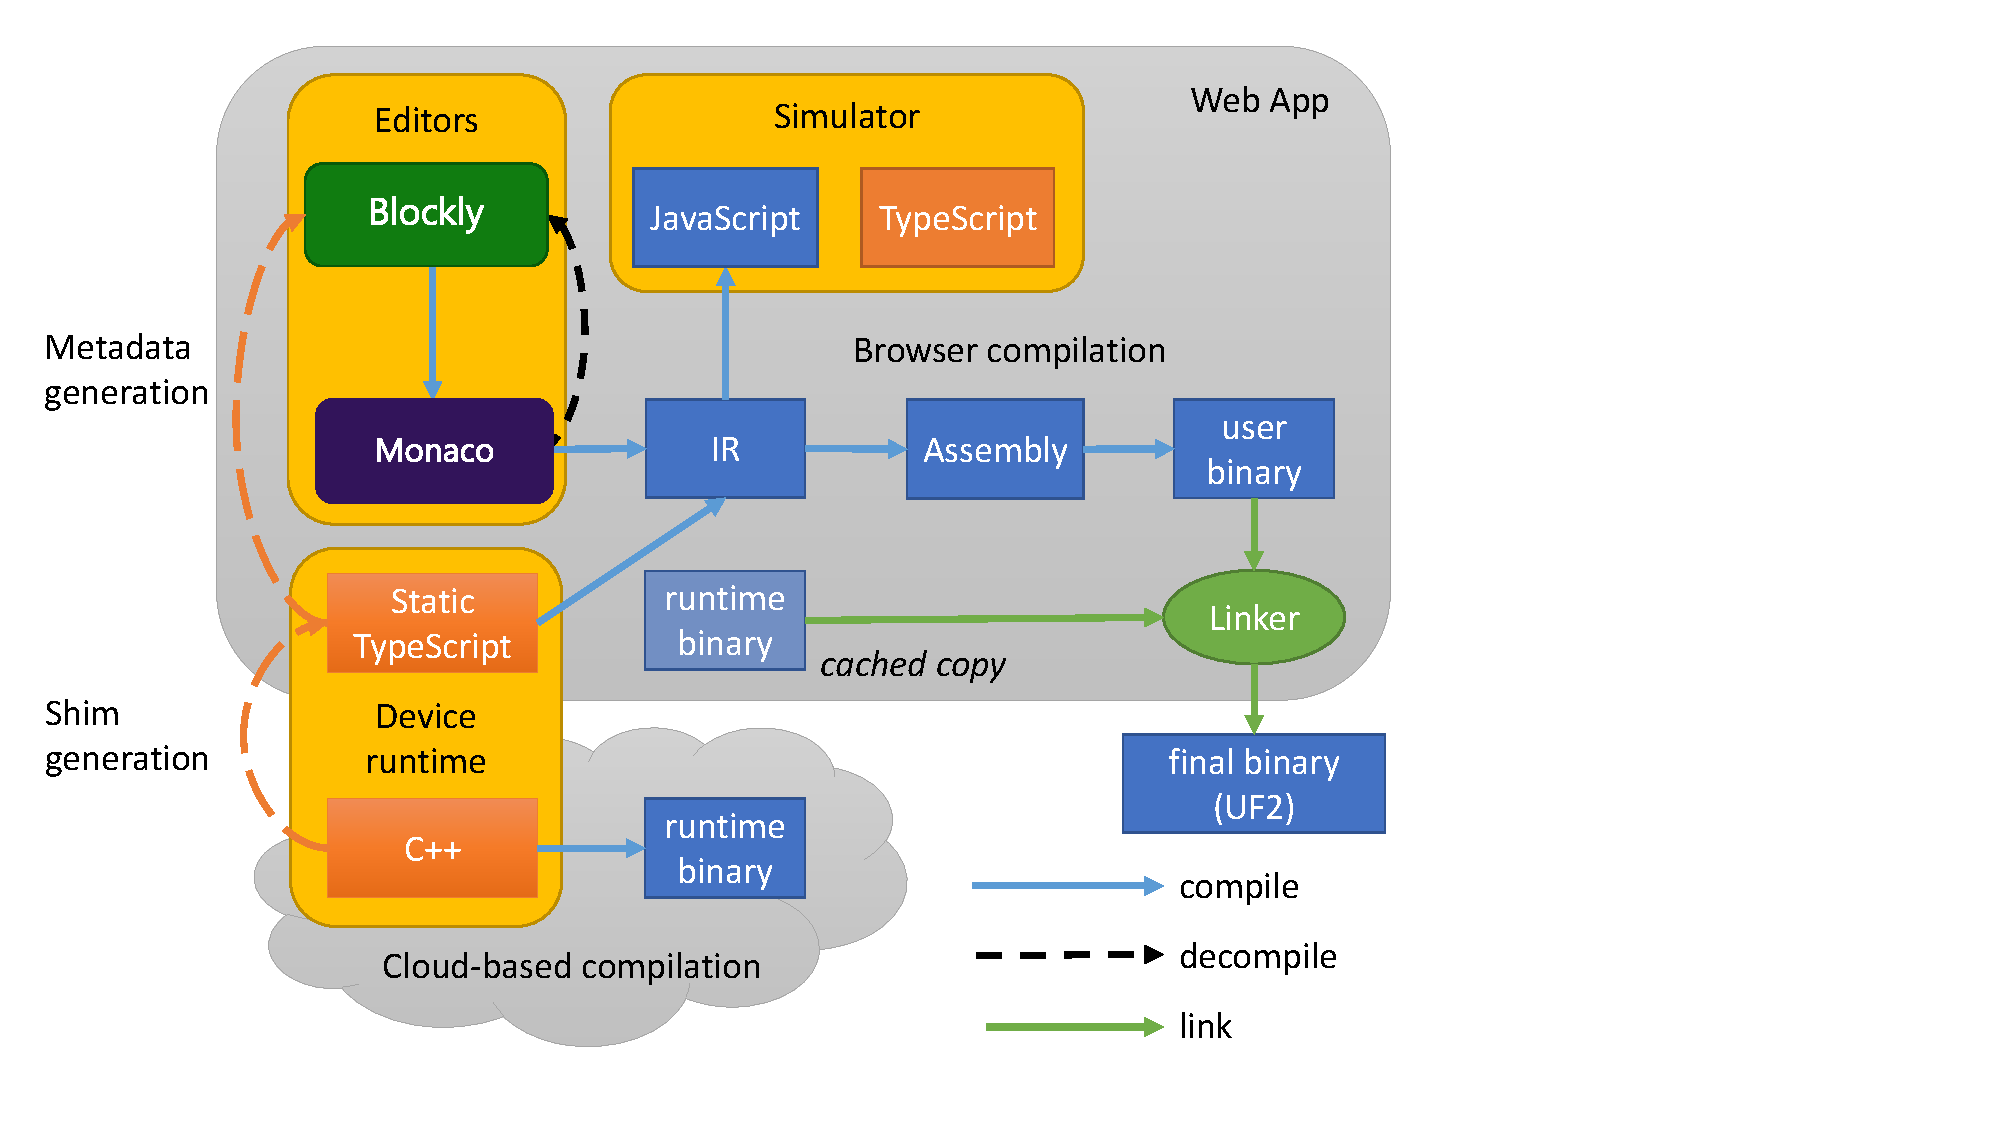
\includegraphics[width=4.5in]{makecodeFig.pdf}
\caption{\label{fig:makecode}\MC Architecture}
\end{figure}

Mapping of functions and enumerations between C++ and TypeScript is straightforward
and performed automatically by \MC. 
Here's an example of the C++ function plot in the led namespace that wraps a more
complex function call of the underlying device runtime to set/plot an LED in the micro:bit display:

\begin{lstlisting}
//% blockId=device_plot block="plot|x %x|y %y"
//% x.min=0 x.max=4 y.min=0 y.max=4
void plot(int x, int y) {
    uBit.display.image.setPixelValue(x, y, 1);
}
\end{lstlisting}

We'll describe the attribute definitions in the \emph{//\%} comment in the next section. 
\MC uses a TypeScript declaration file (here called a shim file) to describe the TypeScript elements corresponding
to C++ namespaces, enumerations and functions.
Since the C++ plot function is preceded by a \emph{//\%} comment, 
\MC adds the following TypeScript declaration to the shim file and copies
over the attribute definitions in the comment. \MC also adds an attribute definition mapping
the TypeScript shim to its C++ function (shim=led::plot):

\begin{lstlisting}
//% block="plot|x %x|y %y
//% shim=led::plot
function plot(x: number, y: number): void;
\end{lstlisting}

The following TypeScript code defines a function to toggle the state of a LED
using three functions (led.point, led.unplot, and led.plot) exposed by the C++ runtime:  
\begin{lstlisting}
//% block="toggle|x %x|y %y"
function toggle(x: number, y: number): void {
    if (led.point(x, y)) led.unplot(x, y)
    else led.plot(x, y)
}
\end{lstlisting}
To the end user, the toggle function appears as just another runtime function available
in the LED namespace. 

%Here is the shim file generated from C++ micro:bit device runtime:
%\dbhref{https://github.com/Microsoft/pxt-microbit/blob/master/libs/core/shims.d.ts}{pxt-microbit/libs/core/shims.d.ts}.

To support the foreign function interface, \MC defines a mapping between C++ and TypeScript types.
Boolean and void have straightforward mappings from C++ to TypeScript (bool $\rightarrow$ boolean, void $\rightarrow$ void). 
As JavaScript only supports number, which is a C++ float/double, \MC uses TypeScript's support
for type aliases to name the various C++ integer types commonly used for microcontroller programming
(int32, uint32, int16, uint16, int8, uint8). 
% don't use int, unsigned etc. they are actually different sizes on different compilers for AVR
This is particularly useful for saving space on 8-bit architectures such as the AVR. 

%\MC allows a set of C++ functions with the same first parameter (of type Foo) to be
%exposed as a TypeScript interface Foo as follows: this set of C++ functions must be grouped
%inside a namespace of the name FooMethods.  
%See, for example, how a C++ buffer abstraction is exposed in TypeScript:
%\dbhref{https://github.com/Microsoft/pxt-microbit/blob/master/libs/core/buffer.cpp}{pxt-microbit/libs/core/buffer.cpp}.
%You can find the resulting TypeScript Buffer interface in the previously referenced shim file for the micro:bit.

\MC includes reference counted C++ types for strings, lambdas (with
up to three arguments and a return type), collections, and user-defined classes/records.  
\MC does not yet include garbage collection, so advanced users who create cyclic
data structures must be careful to break cycles in order to ensure complete deallocation. 

\subsection{Metadata generation}

Both C++ and TypeScript APIs can be specially annotated (minimally via 
\emph{//\% block}) so that the \MC compiler generates the needed
Blockly metadata to expose an API as a visual block.
Additional attribute definitions can provide text descriptions for the block, project function
parameters (thus simplifying the API available via Blockly), and describe other visual/functional
characteristics of the block.  \MC uses the types of function parameters to select appropriate
Blockly widgets.  For example, an enumeration is represented by a dropdown menu.
%For more information on the block-specific annotations, see 
%\dburl{https://makecode.com/defining-blocks}. 
\MCN's support for Blockly means that for the common case, the target developer doesn't need
to know anything about the Blockly framework.
For more sophisticated needs, one can directly access the Blockly framework. 

\subsection{Editors}

As shown in the upper-left of Figure~\ref{fig:makecode},
\MC uses the Blockly (\emph{\href{https://github.com/google/blockly}{blockly}}) and Monaco 
(\emph{\href{https://github.com/Microsoft/monaco-editor}{monaco-editor}}) editors to allow the user to code with
visual blocks or TypeScript. The editing experience is parameterized by the full-typed device
runtime, which provides a set of categorized APIs to the end-user, based on namespaces, as
previously described. These APIs are visible in both editors via a toolbox (Figure~\ref{fig:screenSnap}(C))
to the immediate
left of the programming area. The Blockly and Monaco toolboxes show the same set of APIs, to
help in transition from coding with blocks to coding with JavaScript. More advanced TypeScript
APIs can be discovered in Monaco via code intellisense.

\MC compiles the Blockly program representation to Static TypeScript in a syntax-directed manner.
A key issue is the need for type inference on the Blockly representation, as variables generally are defined and used without
being declared in Blockly. \MC uses a simple unification type inference to assign a
unique type to each variable.  
% this may not be possible:
%In the future, we expect to use TypeScript's type inference instead
%and eliminate the need for separate type inference over the Blockly representation. 
TypeScript supports programming constructs that are not available in Blockly, such as classes.
Such constructs are converted into grey uneditable blocks in Blockly, with the construct's program
text intact. This means \MC always can decompile a TypeScript program to Blockly and then recover
the program text of the grey blocks when converting from Blockly back to TypeScript.
% (see \emph{\dbhref{https://github.com/Microsoft/pxt/blob/master/pxtcompiler/emitter/decompiler.ts}{decompiler.ts}}). 

\subsection{Browser compilation}

\MC first invokes the TypeScript language service to perform type inference and type checking on the 
user's program, the device runtime writen in TypeScript, as well as the TypeScript declarations
corresponding to the C++ device runtime. It then checks that the
combined TypeScript program is within the STS subset through additional syntactic and type checks over the typed AST (detailed in Section~\ref{sec:sts}).  Assuming all the
above checks pass, \MC then performs tree shaking of the AST to remove unused TypeScript functions.
The reduced AST then is compiled to an intermediate representation (IR) that makes explicit: labelled control 
flow among a sequence of instructions with conditional and unconditional jumps; heap cells; field accesses; store operations,
and reference counting.

\flameon{MICHAL: can you please add a little more about the design of IR and the code generation - this PLDI, after all.}

There are three backends for code generation from the IR. The first backend generates JavaScript,
for execution against the simulator runtime.  A second backend generates assembler, parameterized by a
processor description.  Currently supported processors include ARM's Cortex class (Thumb instructions)
and Atmel's Atmega class (AVR instructions). A separate assembler, also parameterized by an instruction
encoder/decoder, generates machine code and resolves runtime references, producing a final binary executable. A third backend generates bytecode instructions.
\MC can encode the resulting binary in a number of formats, 
including Intel's HEX format and the \UF format, introduced in Section~\ref{sec:uf2}.

%The compiler chain
%can be found at \emph{\dbhref{https://github.com/Microsoft/pxt/tree/master/pxtcompiler/emitter}{pxtcompiler/emitter}} and 
%\emph{\dbhref{https://github.com/Microsoft/pxt/tree/master/pxtlib/emitter}{pxtlib/emitter}}.


\subsubsection{Asynchronous Functions}

An important part of the compilation process is to allow users to call asynchronous 
TypeScript functions (identified through the \emph{//\% async} annotation) 
as if they were blocking functions.  For example, in Figure~\ref{fig:example}, the runtime 
function \emph{basic.pause(1000)} (called at line 10) 
is an async function that sets a countdown timer (for 1000 milliseconds) 
and then yields to the scheduler. When the timer 
reaches zero, the function continuation is queued for execution. 

For execution in the single-threaded context of the JavaScript runtime,
every TypeScript function is compiled so that it can be suspended (at the return of a call) and later resumed (at the same point). 
The default behavior at a suspension point is to immediately resume execution.  For a call to an async function,
the default behavior is overridden by the compiler, which suspends execution of the current function. 
Upon completion of the async function call, the current function then is resumed. 
The \CO device runtime supports fibers with the ability to yield, so for compilation to a device, 
the compiler simply emits a call to yield at a suspension point.

Async functions are written by runtime developers, not end-users, and greatly simplify the JavaScript
programming model for end-users. For example, although the JavaScript simulator runtime uses promises to 
achieve asynchronous execution in a single-threaded context, these promises are hidden from the end user. 

\subsubsection{Untagged and Tagged Strategies}

The \MC compiler supports the Static TypeScript language subset described in Section~\ref{sec:sts},
with two compilation strategies: untagged and tagged. Under the untagged strategy,
a JavaScript number is interpreted as a C++ int by default and the type system is used
to statically distinguish primitive values from boxed values. As a result, the untagged
strategy is not fully faithful to JavaScript semantics: there is no support for floating
point and the Null and Undefined types are represented by the default integer value of zero.

The untagged strategy is used for the micro:bit and Arduino Uno targets. For example,
in line 11 of the micro:bit program in Figure~\ref{fig:example}, the division and modolu 
operations are integer operations. 

In the tagged strategy, numbers are either tagged 31-bit signed integers, or if they do not fit, 
boxed doubles. Special constants like false, null and undefined are given special values 
and can be distinguished. The tagged execution strategy has the capability to fully support
JavaScript semantics. This strategy is used for all SAMD21 targets.

\subsection{Simulator}

A \MC target can provide an alternate TypeScript implementation for each API in the device runtime, for use in the device
simulator. As this code runs in the web browser (not on the actual device) and manipulates the DOM, the developer is free to
use all of TypeScript/JavaScript's features. (As an aside, \MC also support ``simulator-only'' targets that have no 
associated device; in these cases, the ``device runtime'' is defined solely by the simulator APIs.) 

As shown in Figure~\ref{fig:screenSnap}(B), the simulator allows the user to experience the basic functions of the device 
in the browser and to test their code
before deploying it to the actual device. The simulator has proxy widgets for sensors such as accelerometer (mouse motion),
temperature and light, allowing the user to control the sensor's value.  The simulator only provides basic functionality
and is far from a complete device emulation.  
% For example, it is not possible for the user to simultaneously modify two
%inputs to the simulated device, while it is possible with the actual device (i.e., shaking it to change the accelerometer
%reading while pushing one of the device's buttons).

%\MC provides various components to make device simulators easier to build: board, parts, wiring, etc.

